% !TEX program = arara
% arara: pdflatex
% arara: biber
% arara: pdflatex
% arara: pdflatex
% arara: clean: { files: [ Paper.out ] }
% arara: clean: { files: [ Paper.aux, Paper.bbl ] }
% arara: clean: { files: [ Paper.bcf, Paper.blg ] }
% arara: clean: { files: [ Paper.log, Paper.run.xml ] }
% arara: clean: { files: [ Paper.toc, Paper-blx.bib ] }
% 

\documentclass{Paper}
%\usepackage{todonotes}
\usepackage{xcolor}
\usepackage{float}
\usepackage{textcomp}
\usepackage{subfigure}
\usepackage{filecontents}



\begin{document}

\maketitle

% % % % %

\tableofcontents
\clearpage

\section*{Abstract}\addcontentsline{toc}{section}{Abstract}
	\textit{Autor: Berna, Überarbeitung: Jana}\\
Das Ziel dieses Projekts ist festzustellen, wie sich menschliche Zeitwahrnehmung in der Virtual Reality durch visuelle und akustische Zeitgeber manipulieren lässt und ob sich die Zeitwahrnehmung auch in der realen Welt nach einem Aufenthalt in der VR verändert.\\
Dazu legten Versuchspersonen Zeiteinschätzungstest ab und wurden daraufhin in einer virtuellen Testumgebung und unwissend über die Forschungsfragen sowohl langsamen als auch schnellen Zeitgebern ausgesetzt. 
Die persönliche Einschätzungen zur vergangenen Zeit hielten die Versuchspersonen anschließend in einem Fragebogen fest. Es wurden weitere Zeiteinschätzungstests durchgeführt und mit den Ergebnissen vor der VR verglichen, um Veränderungen in der Zeitwahrnehmung festzustellen (unter Berücksichtigung verschiedener Störfaktoren).\\
\textbf{hier Ergebnisse einfügen, sofern welche vorhanden}



\section{Einleitung}

\subsection{Einstieg}
\textit{Autor: Kim, Überarbeitung: Jana}\\
In den letzten Jahrhunderten ist ein enormer Wandel unserer Gesellschaft auf technischer und sozialer Ebene zu beobachten. Gleichermaßen ist eine erhöhte Relevanz des Begriffes \textit{Zeit} durch vermehrte öffentlichen Diskussionen über Krankheiten wie Stress und Burn-Out zu beobachten. Immer mehr Menschen leiden an diesen Krankheiten, die auf ,,zu wenig Zeit'' zurückzuführen sind. Das zunehmende Interesse der Themen Effizienz, Schnelligkeit und Leistung ist unübersehbar. 
%Die Gesellschaft versucht immer schneller und immer mehr Arbeiten in einer kürzeren Zeit zu erledigen. 
Dies ist auch auf die Industrialisierung und das zunehmende Tempo der Gesellschaft zurückzuführen. \cite{Wallisch2003} Wo früher noch Tage auf die Antwort eines Briefes gewartet wurde, ist es heute innerhalb weniger Minuten möglich ganze Arbeitsschritte oder Anweisungen digital zu kommunizieren und anschließend die erwarteten Leistungen zu erbringen.
Des Weiteren lässt sich beobachten, dass die Arbeits- und Schlafzeiten der arbeitenden Bevölkerung massiv gesenkt wurden. \cite{DeutscheSozialgeschichte}
\\
Aufgrund von weniger Schlafzeiten ergibt sich nun die Bildung der Freizeit und somit die Notwendigkeit des Zeitmanagements. Jeder versucht seine Tage optimal zu nutzen und einzuteilen, um noch genug Zeit für die Freizeit und Familie zu haben. Des Weiteren schaffen auch die neuen Entwicklungen der Industrialisierung wie Handy, Mikrowelle, Computer und weitere technische Erfindungen mehr Zeit für jeden Einzelnen. Dennoch sind Versuche, die Zeit durch immer effizientere und „zeitsparendere“ Abläufe zu bändigen nur Scheinerfolge: Die Zeit vergeht trotzdem gleichförmig und unaufhaltsam und unwiderruflich weiter. \cite{Wallisch2003} Es besteht also ein hohes Interesse in der Erforschung dieses Gebietes, um die Zeit, die jedem Einzelnen zur Verfügung steht, optimal zu nutzen.

Dem Menschen steht immer noch derselbe biologische Apparat zur Verfügung, Zeit vergeht also trotzdem gleichförmig und einheitlich. Doch ist das wirklich so oder gibt es bestimmte Indikatoren, die uns die Zeit als schneller oder langsamer vergehend vorkommen lassen? Kann man das Zeitempfinden also beeinflussen?

\subsection{Fragestellung und Hypothesen}
\textit{Autor: Kim, Überarbeitung: Jana}\\
Daraus entwickelt sich die Fragestellung dieser Arbeit: ,,Wie stark lässt sich das menschliche Zeitempfinden durch in der VR eingesetzte visuelle und auditive Zeitgeber manipulieren und wie nachhaltig ist der Einfluss eines Aufenthalts in der VR auf das menschliche Zeitempfinden im realen Leben?''\\
Als Zeitgeber sind hier Phänomene der allgemeinen Lebenswelt und physische Kräfte definiert, die unter Ausschluss der Uhrzeit die Zeit vorgeben.\\
Von oben genannter Fragestellung ausgehend werden in dieser Arbeit zum einen \textit{Hypothese 1:} ,,Innerhalb der VR erlebte visuelle und auditive Zeitgeber verfälschen das Zeitempfinden einer Person entsprechend der gewählten Schnelligkeit'' und darüber hinaus \textit{Hypothese 2:} ,,Nach einem Aufenthalt in der VR ist das menschliche Zeitempfinden auch in der realen Welt verändert'' auf ihre Gültigkeit überprüft.
 
\subsection{Forschungsstand}
\textit{Autor: Kim, Überarbeitung: Jana}\\
Der Aufbau dieses Projekts berücksichtigt die Ergebnisse dreier Studien zu menschlicher Zeitwahrnehmung und und Zeitmanipulation in der VR.\\
Die Studie ,,Could Virtual Reality Help Manipulate Time Perception?'' einer Forschungsgruppe der Universität Hamburg untersucht menschliche Zeitwahrnehmung in der VR unter verschiedenen Bedingungen. Ein Drittel der Versuchspersonen hält sich passiv in der VR auf, ein weiteres Drittel hat während des Aufenthalts sprachlich kognitive Aufgaben zu lösen und das restliche Drittel räumlich kognitive. 
Als Zeitgeber wird die Sonne verwendet, jeweils in einem von drei verschiedenen Modi: ohne Bewegung, im normalen 24-Stunden-Zyklus und doppelt so schnell wie in der Realität. Die Ergebnisse zeigen, dass die Sonne als Zeitgeber lediglich einen Einfluss auf die Zeitwahrnehmung der Versuchspersonen hat, die in der VR passiv blieben. Ist eine Versuchsperson hingegen mit einer Aufgabe beschäftigt, kann kein Einfluss des Zeitgebers festgestellt werden.\cite{DeviceSystems2016}\\
Aufgrund dieser Erkenntnisse wurden für dieses Projekt keine Aufgaben innerhalb der VR integriert, sodass sichergestellt werden kann, dass die Versuchspersonen nicht von der Beeinflussung der visuellen und akustischen Zeitgeber abgelenkt sind.\\
Pascal Wallisch' wissenschaftlicher Bericht ,,Zeiterleben in der Tempogesellschaft'' nennt Intelligenz, Alter, Geschlecht, Drogen- und Medikamenteneinflüsse, Müdigkeit, Körpertemperatur, Gehirnschäden und psychische Erkrankungen als mögliche interne Einflussfaktoren auf die Zeitwahrnehmung.\cite{Wallisch2003} 
Anhand eines Fragebogens werden diese Faktoren individuell erfasst und können bei der Auswertung berücksichtigt werden.\\
Weiterhin hat auch der Spaßfaktor einen Einfluss auf die Zeitwahrnehmung, der gesondert beachtet werden muss, wie der Artikel ,,Warum Jahre rasen und Sekunden schleichen'' von Rüdiger Schacht zeigt. \cite{Welt24}

\section{Methode}

        %\subsection{Methodik}
        %Die Durchführung des Experiments mit Versuchspersonen, Tests vor und nach der VR und Fragebögen ist die wissenschaftliche Methode dieses Projekts und die Grundlage, anhand derer die Leitfrage und Hypothesen  untersucht und Zusammenhänge dargestellt werden. Das Experiment und seine Durchführung baut auf bereits vorhandenen Forschungen auf und berücksichtigt deren Erkenntnisse.
%Da die Forschung über menschliches Verhalten ethische Schwierigkeiten birgt, wenn es sich um Manipulationen an den Versuchspersonen handelt, wurden bei der Ausführung dieses Projekts auf vertretbare ethische Richtlinien geachtet. D.h. konkret, dass die Versuchspersonen im Vorfeld über den Ablauf des Verfahrens informiert und über die vorhersehbaren Unannehmlichkeiten und die Risiken aufgeklärt wurden. Es bestand jederzeit die Möglichkeit das Experiment abzubrechen.


\subsection{Aufbau und Begründung}
\label{aufbau}
       \textit{Autor: Nizan, Alina. Überarbeitung: Jana}\\
Die Testumgebung besteht aus vier Szenarien, wobei jedes Szenario aus einer Ampelkreuzung und einem Zeitgeber besteht. Es werden insgesamt zwei visuelle und zwei auditive Zeitgeber verwendet, wobei davon jeweils einer schnell und einer langsam ist.
Um eine Beeinflussung durch eine festgelegte Reihenfolge der Szenarien auszuschließen, werden alle möglichen Szenarioreihenfolgen von gleichmäßig vielen Versuchspersonen durchlaufen.

\begin{figure}[H]
	\centering
	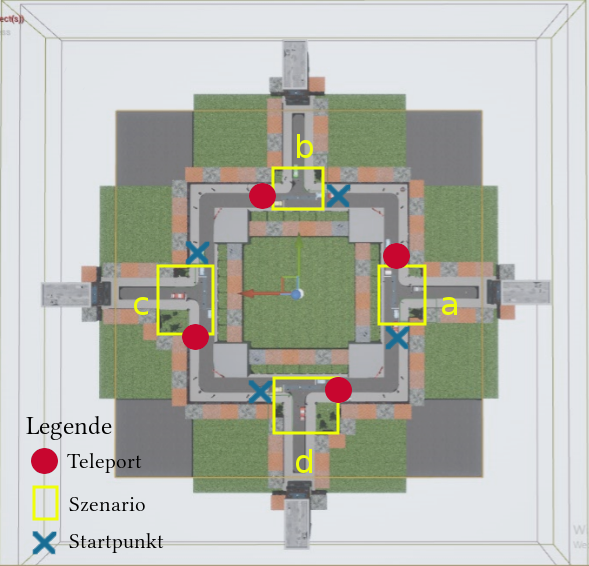
\includegraphics[scale=0.7]{../Bilder/mapLegende.png}
	\caption{Ansicht der Testumgebung von oben}
	\label{img:map}
\end{figure}


Abb. 1 zeigt die Testumgebung von oben. Der Aufbau der Welt ist statisch, sodass ein System aus Teleportern (roter Punkt) die verschiedenen Reihenfolgen der Szenarien ermöglicht. Es gibt vier mögliche Startpunkte (blaues X), wobei pro Durchlauf je nur einer aktiv ist.
Welcher Startpunkt gewählt wird ist von der verwendeten Reihenfolge der Szenarien abhängig. Die Laufrichtung ist entgegen des Uhrzeigersinns vorgegeben und der zu erreichende Endpunkt befindet sich immer jeweils hinter dem letzten durchlaufenen Szenario.\\
Vor jeder Abbiegung in Laufrichtung befindet sich ein Teleporter, der durch eine Triggerbox aktiviert wird und die Versuchsperson an die gewünschte Stelle der Karte befördert, wobei alle Teleporter beliebig miteinander verbunden werden können. Durch die immer gleichaussehenden Ecken der Karte wird das Immersionserlebnis der Versuchsperson nicht behindert. 




\begin{figure}[H]

	\subfigure[Ampelphase an einem LKW]{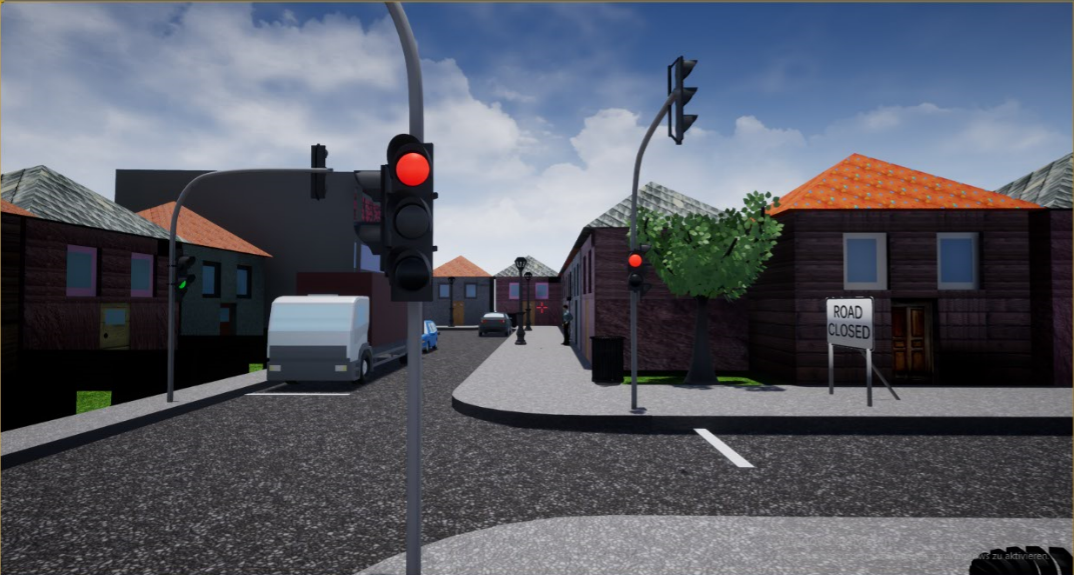
\includegraphics[width=0.5\textwidth]{../Bilder/a.png}}
	\subfigure[Ampelphase mit Vogel und Menschen]{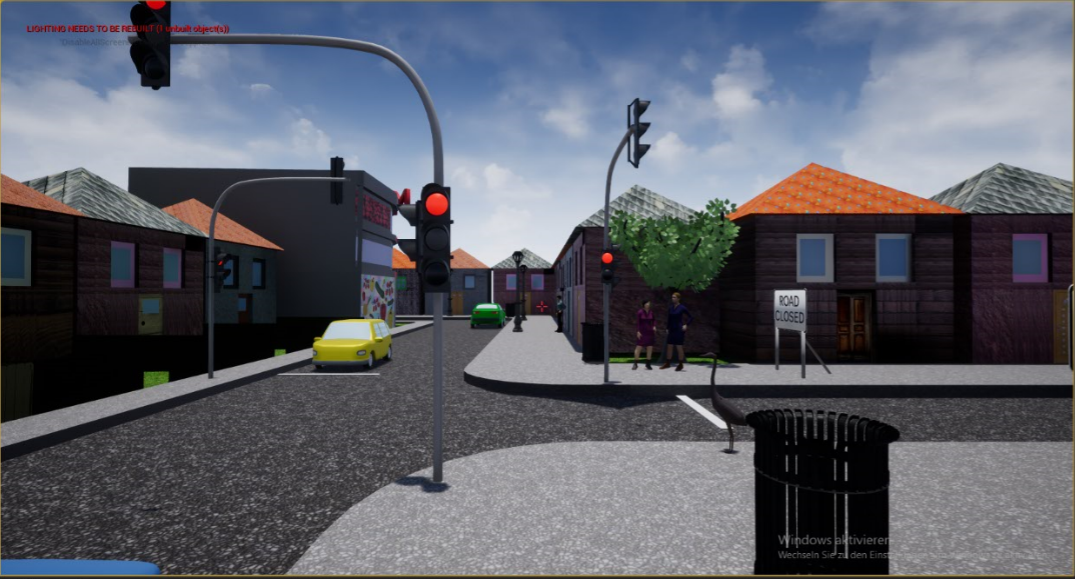
\includegraphics[width=0.5\textwidth]{../Bilder/b.png}}


	\subfigure[Ampel neben einem schaukelndem Kind mit rosa Shirt]{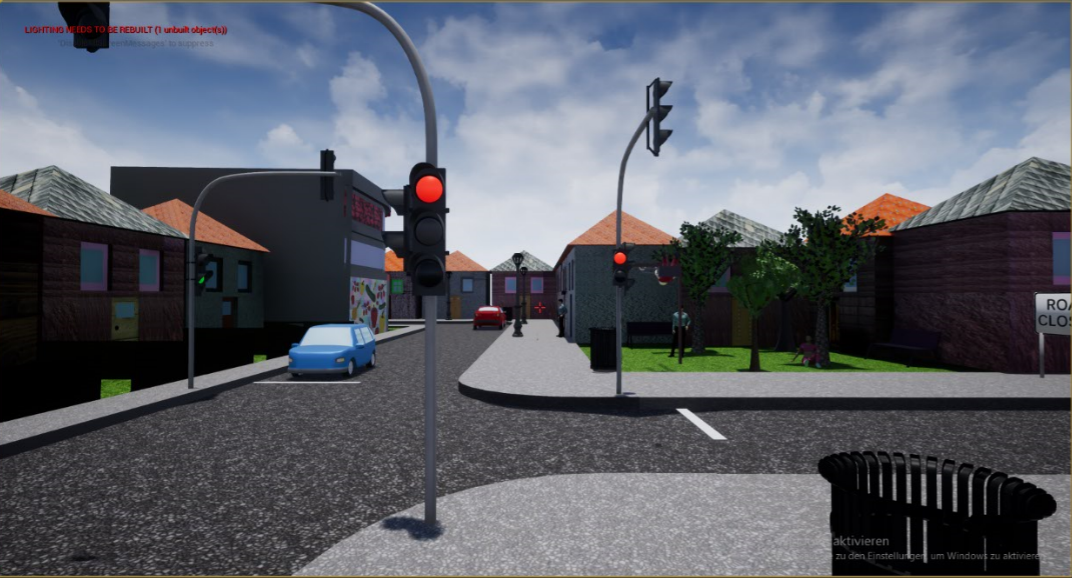
\includegraphics[width=0.5\textwidth]{../Bilder/c.png}}
	\subfigure[Ampel neben einem schaukelndem Kind mit grünem Shirt]{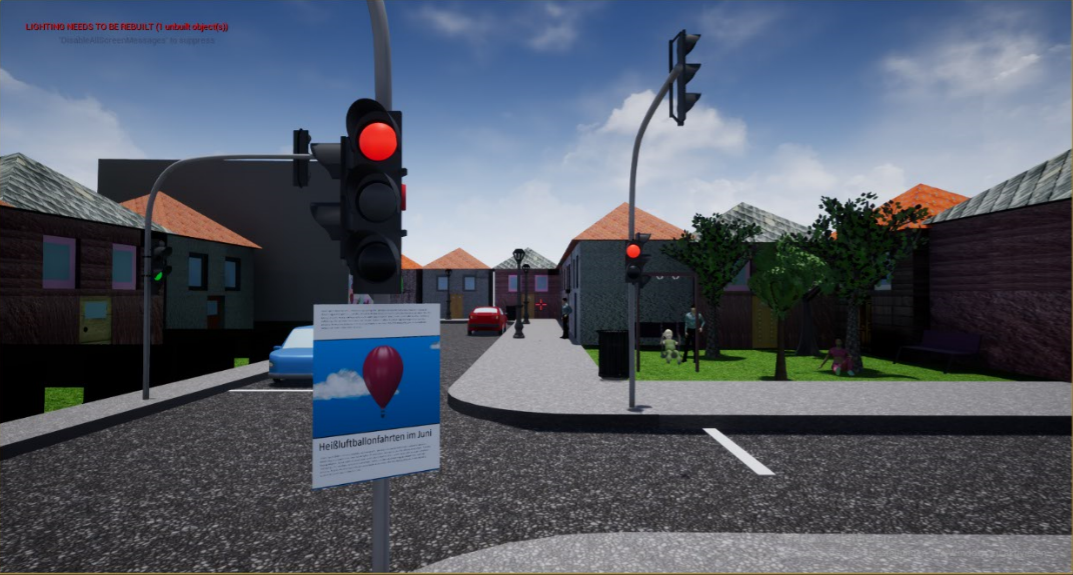
\includegraphics[width=0.5\textwidth]{../Bilder/d.png}}
	\caption{Benutzeransicht der Kreuzungen}
	
\end{figure}

%\label{img:ampelphasen-1} = label{img:ampelphasen}


Das gleichmäßige schnelle (Szenario \textbf{a}) oder langsame (Szenario \textbf{b}) Ticken der Fußgängerampel stellt die auditive Manipulation dar. Um die Erinnerung an die Szenarien zu erleichtern werden auffällige Objekte in den jeweiligen Szenarien verwendet: ein LKW (Szenario \textbf{a}) und ein Fischreiher auf dem Fußgängerweg (Szenario \textbf{b}).
Die visuelle Zeitmanipulation wird durch ein schaukelndes Kind realisiert, das durch entsprechende Animationen den Eindruck macht, schneller (Szenario \textbf{c}) oder langsamer (Szenario \textbf{d}) zu schaukeln als es in der Realität möglich ist. Diese Szenarien sind von der Ampel aus gut zu beobachten und können so auf Versuchspersonen wirken.\\
Die Wartezeit jedes Szenarios beträgt 18 Sekunden und basiert auf zuvor gemessenen realen Ampelzeiten. Über eine Triggerbox wird die Ampelschaltung aktiviert, sobald sich die Versuchsperson entsprechend genähert hat. Die Wartezeit ist einerseits kurz genug, um keine Ungeduld hervorzurufen und andererseits lang genug, dass die Versuchspersonen die Möglichkeit haben sich auf ihre Umgebung einzulassen. 

\subsection{Versuchspersonen}
        \textit{Autor: Nizan, Alina. Überarbeitung: Jana}\\
Das Experiment wurde mit insgesamt 48 Versuchspersonen unterschiedlicher akademischer Grade und Berufe  durchgeführt, wobei 35 männlich und 13 weiblich sind und sich im Alter zwischen 17 und 80 Jahren befinden. 
Die insgesamt 24 verschiedenen Reihenfolgen der Szenarien können mit dieser Anzahl zwar realisiert werden, allerdings mussten fünf Versuchspersonen aufgrund von unvollständigen Angaben von der Auswertung ausgeschlossen werden. 
Alle Versuchspersonen hatten nach eigenen Angaben normale oder mit Brille bzw. Kontaktlinsen korrigierte Sehkraft und normales Farbsehen. Die Versuchspersonen waren bezüglich der experimentellen Hypothesen unwissend und unterschrieben vor der Teilnahme eine Einverständniserklärung, die sie auf mögliche Risiken einer VR-Nutzung aufmerksam machte. Es wurde keine Entschädigung angeboten. 

        \subsection{Apparaturen}
                \textit{Autor: Nizan, Alina. Überarbeitung: Jana}\\
Zwei Räume wurden für die Durchführung des Experiments genutzt, wobei im ersten alle Befragungen und Tests stattfanden und im zweiten die virtuelle Testumgebung aufgebaut war.\\
Zu den Materialien des ersten Raumes gehören die Einverständniserklärung, die von der Versuchsperson auszufüllenden Fragebögen A und C und der Intelligenztest.
Die Versuchsleiter nutzen in diesem Raum eine Stoppuhr für Zeiteinschätzungstests, ein Infrarot-Thermometer und Fragebogen B, um die ermittelten Werte festzuhalten.
Bei dem angewandten Intelligenztest handelte es sich um den psychologisch anerkannten ,,Mehrfach-Wortschatz-Test (MWT-B)'', entwickelt von Siegfried Lehrl \cite{MWT-B}. Dieser Test ist vergleichsweise simpel und kurz durchzuführen und bietet einen groben Überblick über die allgemeine Intelligenz einer Person. 
%Im MWT-B gilt es aus 37 Wortreihen, welche jeweils aus vier fiktiven und einem existierendem deutschen Wort bestehen, das echte Wort durchzustreichen. Es gibt keine zeitliche Begrenzung oder Hilfestellung.\\
Im zweiten Raum wurde das VR-Experiment durchgeführt, daher befinden sich in diesem Raum eine Oculus Rift (DK2), On-Ear-Kopfhörer und ein Computer, auf welchem sich die mithilfe der Unreal Engine erstellte Testumgebung durchlaufen lässt. Weiterhin wurde zur Steuerung ein Xbox-Controller verwendet. Die Versuchsleiter messen die tatsächlich verbrachte Zeit in der VR mit einer Stoppuhr.
\subsection{Prozedur}
        \textit{Autor: Nizan, Alina. Überarbeitung: Jana}\\
Der Ablauf des Experiments besteht aus drei Phasen: Intelligenztest und erste Zeiteinschätzungen, Navigation durch die virtuelle Testumgebung, Zweite Einschätzungen.
\subsubsection{Intelligenztest und erste Zeiteinschätzungen}

Der erste Teil des Experiments fand in \textit{Raum 1} statt, in welchem sich Versuchsleiter und die Versuchsperson gegenüber sitzen.\\
Nach Unterschreiben der Einverständniserklärung wurde der erste von insgesamt sechs Zeiteinschätzungstests durchgeführt, in welchem die Versuchsperson 40 Sekunden ohne Gespräch abzuschätzen hat. Die Versuchsperson gibt auf Fragebogen A alle für das Experiment relevanten internen Einflussfaktoren (vgl. Kapitel 1.3  Forschungsstand) an.
Danach werden der Intelligenztest und der zweite Zeiteinschätzungstest (40 Sekunden während eines Gesprächs mit dem Versuchsleiter) durchgeführt. Die Körpertemperatur der Versuchsperson wird anschließend mithilfe eines Infrarot-Thermometers am Ohr gemessen und der dritte Zeiteinschätzungstest (30 Sekunden ohne Gespräch) durchgeführt.
Alle Ergebnisse der Zeiteinschätzungen und die
Körpertemperatur werden von dem Versuchsleiter auf Fragebogen B notiert, in welchen die Versuchsperson keine Einsicht hat.

\subsubsection{Navigation durch die virtuelle Testumgebung}
Die zweite Phase findet in \textit{Raum 2} statt. Der Versuchsperson werden VR-Brille und Kopfhörer aufgesetzt, danach wird sie in die Steuerung durch den Xbox-Controller eingewiesen und auf generelle Regeln innerhalb der VR aufmerksam gemacht (Gehwege können nicht verlassen werden, es gibt einen zu erreichenden Endpunkt, allgemeine Verkehrsregeln wie das Warten an einer roten Ampel müssen beachtet werden). 
Die Zeit, die die Versuchsperson vom Beginn des Loslaufens bis zum Erreichen des Endpunkts benötigt, wird festgehalten.
Die Versuchsperson durchläuft die Testumgebung einmal, ohne zeitliche Begrenzung und ohne Unterbrechungen. Die Geschwindigkeit kann sie mithilfe des Controllers selbst bestimmen. Die Versuchsleiter können das Geschehen in der VR über einen Monitor beobachten.

\subsubsection{Zweite Einschätzung}
Nach Durchlaufen der Testumgebung wird die Versuchsperson, zurück in \textit{Raum 1}, auf Einflüsse der VR getestet. Ein weiteres Mal schätzt sie die Zeit ab (40 Sekunden ohne Gespräch) und gibt weitere Einschätzungen zur VR auf Fragebogen C an. Dazu gehören (1) die geschätzte Dauer einzelner Szenarien, (2) das jeweils als beste und als schlechteste empfundene Szenario, (3)  die empfundene Dauer in der VR, (4) den empfundenen Spaßfaktor, (5) Auffälligkeiten in der VR und (6) eine Einschätzung, worum es in dem Experiment ging.
Zum Schluss werden zwei letzte Zeiteinschätzungstest durchgeführt (40 Sekunden mit Gespräch, dann 30 Sekunden ohne Gespräch) und zur Auswertung notiert.


\section{Ergebnisse}
\subsection{Einfluss der Zeitgeber}
        \textit{Autor: Jovana, Jana. Überarbeitung: Svenja, Jana}\\
Im Folgenden soll zunächst \textit{Hypothese 1} überprüft werden. Um einen Einfluss der verwendeten Zeitgeber festzustellen, wurden die Versuchspersonen darum gebeten, die vier Szenarien der Länge nach zu sortieren und deren jeweilige Zeit in Sekunden anzugeben. Aus diesen Daten kann man herleiten, welches der Szenarien am kürzesten und welches am längsten eingeschätzt wurde und ob diese Einschätzungen mit den erwarteten Wirkungen der Zeitgeber übereinstimmen.
\begin{figure}[H]
\begin{minipage}[t]{0.49\linewidth}
	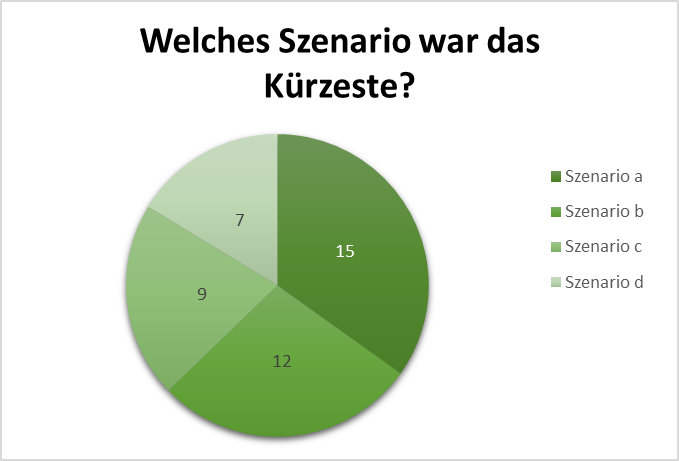
\includegraphics[scale=0.7]{../Diagramme/einschaetzung/kuerzestes.png}
	\caption{Welches Szenario war das kürzeste?}
	\label{SzenarienKurz}
\end{minipage}
%\end{figure}
\hfill
%\begin{figure}[H]
\begin{minipage}[t]{0.49\linewidth}
	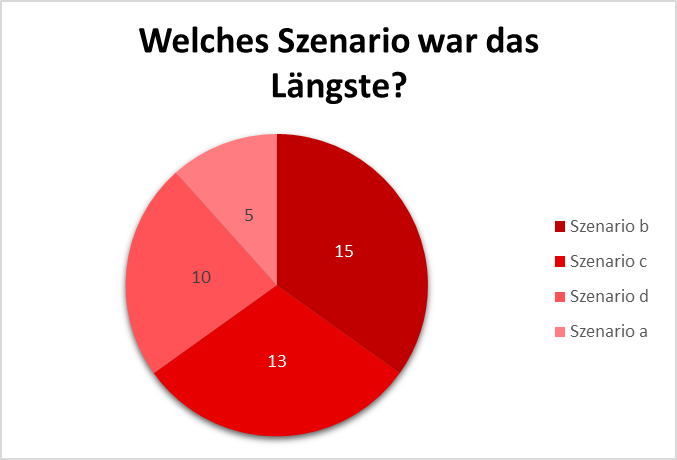
\includegraphics[scale=0.7]{../Diagramme/einschaetzung/laengstes.png}
	\caption{Welches Szenario war das längste?}
	\label{SzenarienLang}
\end{minipage}
\end{figure}

Auffällig ist, dass es bei den meisten Szenarien keine eindeutige Meinung gibt, ob es länger oder kürzer war als die anderen. Einzig bei Szenario \textbf{a} gaben knapp 35\% der Versuchspersonen an, es sei das kürzeste gewesen und nur ca. 12\% behaupten das direkte Gegenteil. 
Betrachtet man allerdings Szenario \textbf{c}, geben die Meinungen kein solch eindeutiges Bild, da es 21\% der Versuchspersonen als das kürzeste, aber 30\% als das längste einschätzen.  Noch extremer ist die Verteilung bei Szenario \textbf{b} (ca. 28\% bewerten es als das kürzeste und 35\% als das längste) und Szenario \textbf{d}  (ca. 16\%  schätzen es als das kürzeste, 23\% als das längste). Betrachtet man die Szenarien getrennt nach akustischen und visuellen Zeitgebern, ergibt sich folgende Verteilung:

\begin{figure}[H]
\begin{minipage}[t]{0.49\linewidth}
	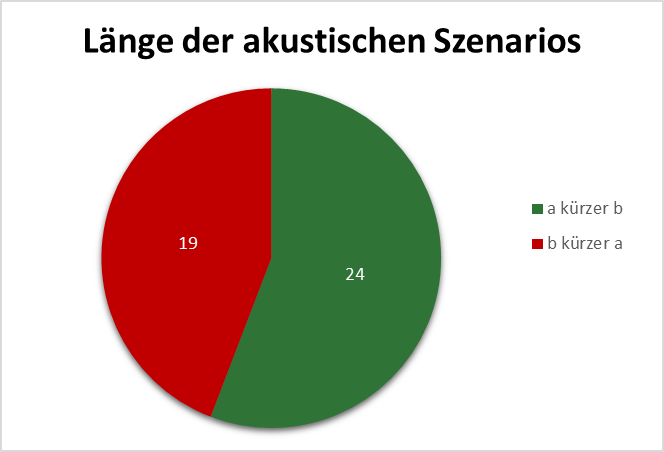
\includegraphics[scale=0.7]{../Diagramme/einschaetzung/laenge_akustisch.png}
	\caption{Längenvergleich der akustischen Szenarien}
	\label{SzenarienAkustisch}
\end{minipage}
%\end{figure}
\hfill
%\begin{figure}[H]
\begin{minipage}[t]{0.49\linewidth}
	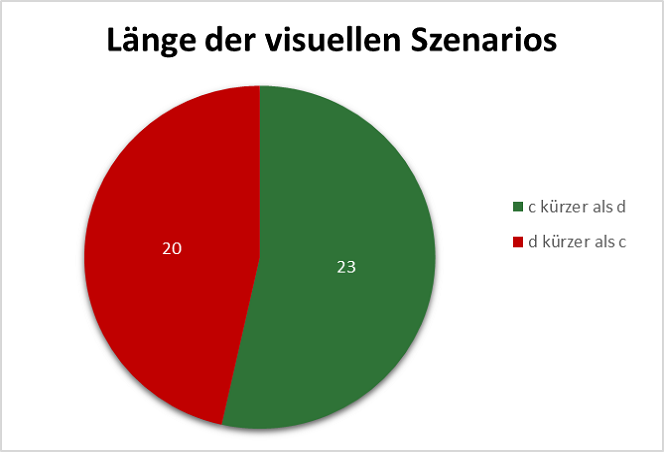
\includegraphics[scale=0.45]{../Diagramme/einschaetzung/laenge_visuell.png}
	\caption{Längenvergleich der visuellen Szenarien}
	\label{SzenarienVisuell}
\end{minipage}
\end{figure}

       
Hier sei nochmal angemerkt, dass die Szenarien \textbf{a} und \textbf{c} die schnellen Zeitgeber enthielten. Durch die akustischen Zeitgeber haben knapp 56\% der Versuchspersonen tatsächlich Szenario \textbf{a} als das schnellere wahrgenommen und ähnliche Ergebnisse gibt es auch bei den visuellen Szenarien: ca. 54\% empfanden Szenario \textbf{c} als schneller. 
Die Szenarien der schnellen Zeitgeber wurden also von der Mehrheit der Versuchspersonen erkannt, allerdings fällt auch hier auf, dass die Verteilung mit jeweils etwas mehr als der Hälfte nicht sehr eindeutig ist. 
      
     \begin{figure}[H]
	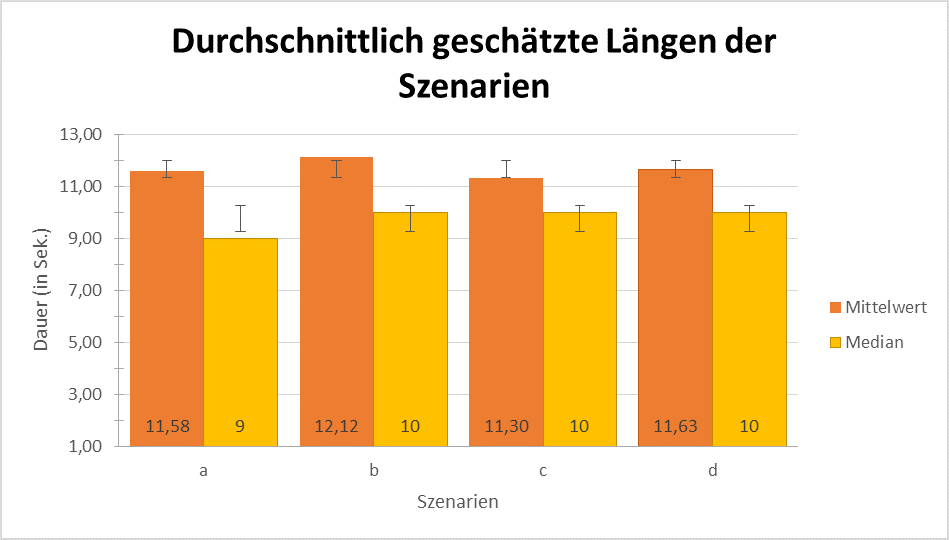
\includegraphics[scale=0.7]{../Diagramme/einschaetzung/laenge_durchschnitt_alle.png}
	\caption{Geschätzte Länge der Szenarien in Sekunden}
	\label{LaengeSzenarien}
\end{figure}

Abb. \ref{LaengeSzenarien} zeigt die durchschnittlich geschätzten Längen jedes Szenarios. Auch hier fällt besonders auf, dass sich die ermittelten Zeiten nur sehr geringfügig voneinander unterscheiden und sich keines der Szenarien als besonders lang oder besonders kurz hervortut, auch wenn die schnellen Zeitgeber nach Abb. \ref{SzenarienAkustisch} und Abb. \ref{SzenarienVisuell} scheinbar ihre Wirkung taten.\\
Aus den Daten lässt sich schlussfolgern, dass die akustischen Zeitgeber eine, wenn auch nur geringfügig, bessere Wirkung auf die Versuchspersonen hatten als die visuellen. Insbesondere zum schnellen Zeitgeber (Szenario \textbf{a}) gab es in denn Abb. \ref{SzenarienKurz} und \ref{SzenarienLang} eine vergleichsweise eindeutige Meinung. Allerdings fällt auch auf, dass die Durchschnittswerte der Abb. \ref{LaengeSzenarien} deutlich unter dem tatsächlichen Zeitwert der Szenarien (18 Sekunden) liegt und weder der Zeitgeber des akustischen noch des visuellen Szenarios die Schätzungen dahingehend manipuliert hat. \\
Entsprechend kann nur ein Teilaspekt der \textit{Hypothese 1} bestätigt werden, da sich Versuchspersonen laut den ermittelten Daten nur vom schnellen akustischen Zeitgeber haben beeinflussen lassen. Weder der schnelle visuelle, noch die langsamen Zeitgeber scheinen eine Wirkung auf die Zeitwahrnehmung der Versuchspersonen zu nehmen. Insbesondere die langsamen Zeitgeber scheinen keinerlei Beeinflussung auf die Versuchspersonen gehabt zu haben, da die entsprechenden Szenarienzeiten deutlich unterschätzt wurden (vgl. Abb. \ref{LaengeSzenarien}).
      
\subsubsection{Spaß als Einflussfaktor}
Im Weiteren soll festgestellt werden, inwieweit Spaß als Einflussfaktor auf die Zeitwahrnehmung eine Rolle spielt.



\begin{figure}[H]
\begin{minipage}[t]{0.49\linewidth}
	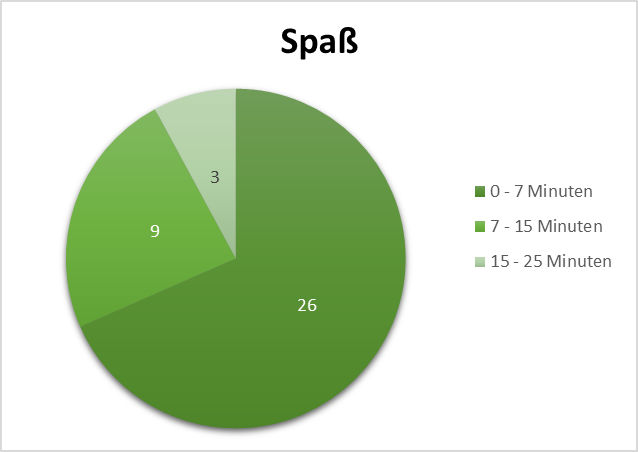
\includegraphics[scale=0.7]{../Diagramme/spass/spass.png}
	\caption{Einschätzung, wie viel Zeit in der VR verbracht wurde (mit Spaß)}
	\label{spass}
\end{minipage}
%\end{figure}
\hfill
%\begin{figure}[H]
\begin{minipage}[t]{0.49\linewidth}
	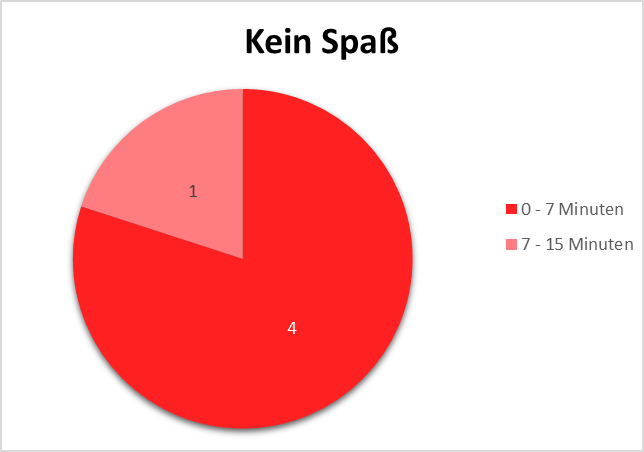
\includegraphics[scale=0.7]{../Diagramme/spass/keinSpass.png}
	\caption{Einschätzung, wie viel Zeit in der VR verbracht wurde (ohne Spaß)}
	\label{keinspass}
\end{minipage}
\end{figure}

Abb. \ref{spass} und \ref{keinspass} zeigen die Einschätzungen der Versuchspersonen, wie viel Zeit sie in der VR verbracht haben. Die Gruppe, die dabei Spaß empfand, gab eine starke Mehrheit von knapp 68\% eine Dauer von 0-7 Minuten an. Aus der andere Gruppe entschieden sich sogar 80\% für dieses Zeitintervall. Da die Intervalle allerdings ungünstig gewählt wurden, bezieht sich dieses Paper im Folgenden und trotz der starken Mehrheit der Angaben nur noch auf die tatsächliche Dauer, die die Versuchspersonen in der VR verbracht haben.


      
     \begin{figure}[H]
	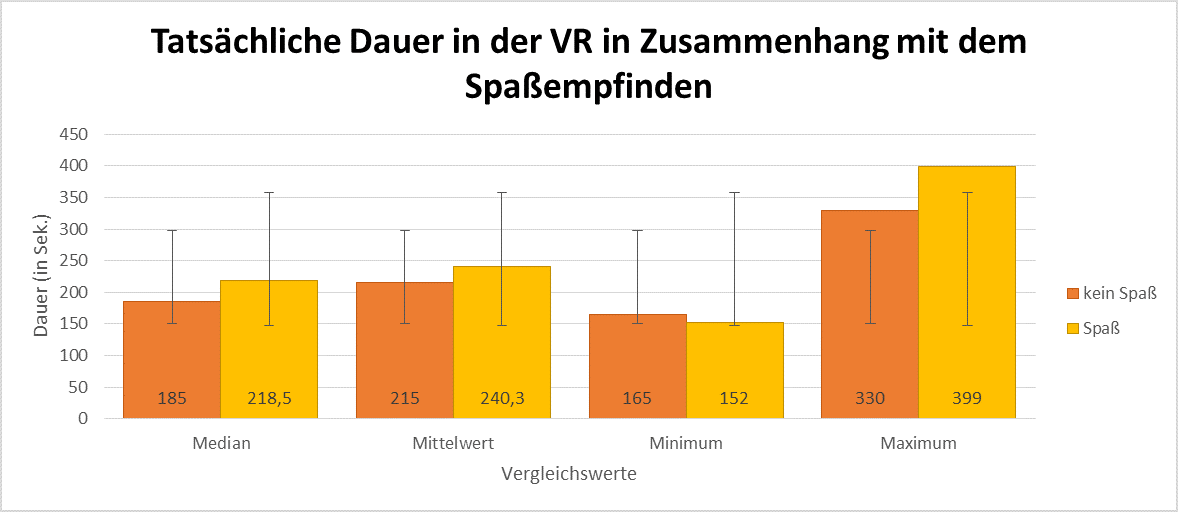
\includegraphics[scale=0.7]{../Diagramme/spass/spassDauer.png}
  \caption{Tatsächliche Zeit, die Versuchspersonen in der VR verbrachten}
  \label{ZeitKeinSpass}
  %DURCHSCHNITT: 212,42 sek
        \end{figure}
        
        Abb. \ref{ZeitKeinSpass} zeigt die tatsächlichen Zeiten, die die Versuchspersonen in der VR verbrachten, getrennt nach Spaß und keinem Spaß. Besonders fällt hier auf, dass die Versuchspersonen, die nach eigenen Angaben keinen Spaß hatten, im Durchschnitt auch tatsächlich weniger Zeit in der VR verbrachten. Einzig das absolute Minimum eines VR-Aufenthaltes gehört zu einer Person, die Spaß hatte. 

\begin{figure}[H]
\begin{minipage}[t]{0.49\linewidth}
	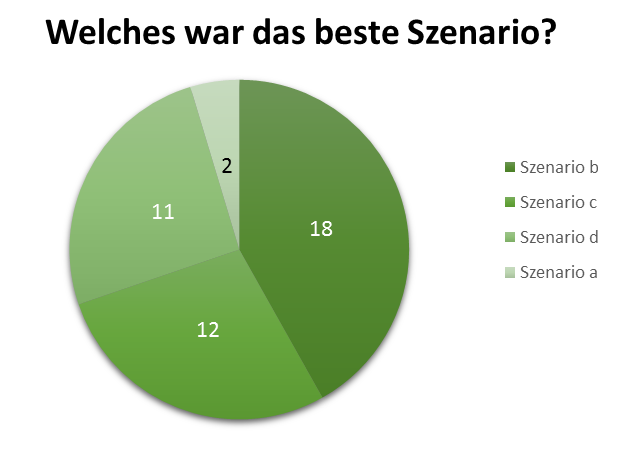
\includegraphics[scale=0.7]{../Diagramme/bewertung/best.png}
	\caption{Welches war das beste Szenario?}
	\label{SzenarioGut}
\end{minipage}
%\end{figure}
\hfill
%\begin{figure}[H]
\begin{minipage}[t]{0.49\linewidth}
	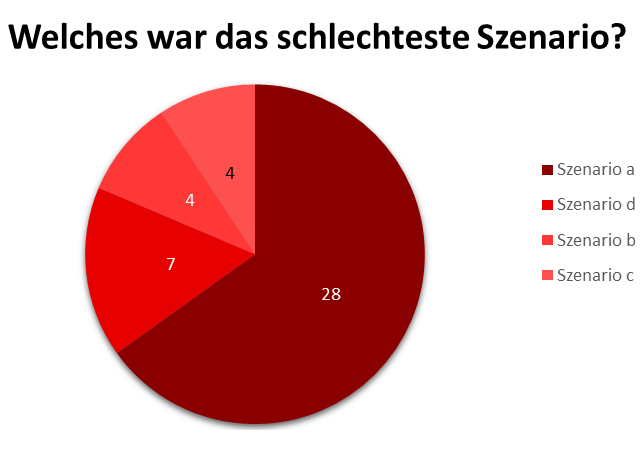
\includegraphics[scale=0.7]{../Diagramme/bewertung/schlecht.png}
	\caption{Welches war das schlechteste Szenario?}
	\label{SzenarioSchlecht}
\end{minipage}
\end{figure}

Nach der Ausgangsvermutung, dass das subjektiv beste Szenario auch das ,,spaßigste'' und damit kürzeste sein müsste, gaben die Versuchspersonen eine Rangfolge der Szenarien ab.\\
Auch hier schneidet insbesondere Szenario \textbf{a} mit einer klaren Meinung ab: nicht einmal 5\% empfinden es als das beste, wohingegen sich 65\% einig sind, es sei das subjektiv schlechteste. Szenario \textbf{b} wird hier eindeutiger bewertet als zuvor, da es knapp 42\% als das beste und 9\% als das schlechteste bewerten. Szenario \textbf{c} (28\% bewerten es als das beste und 9\% als das schlechteste) und Szenario \textbf{d} (26\% bewerten es als das beste und 16\% als das schlechteste) sind ebenfalls, wenn auch nicht in dem Maße wie die ersten beiden, recht eindeutig verteilt. 
Nach der These, dass das bestbewertetste Szenario auch das subjektiv kürzeste ist, müsste die meistgewählte Reihenfolge \textbf{b c d a} sein. 
Die tatsächlich angegebene Reihenfolge hingegen ist allerdings \textbf{a b c d} (vgl. Abb. \ref{SzenarienKurz}).
In diesem Zusammenhang kann die These, dass bei Spaßempfinden die Zeit gefühlt schneller vergeht, nicht bestätigt werden, da insbesondere auch das schlechtbewertetste Szenario \textbf{a} wurde als eindeutig kürzeste gewählt wurde. 

\subsection{Einfluss der VR auf das Zeitempfinden}
\subsubsection{Zeitschätzungen vor der VR}
Im Folgenden soll \textit{Hypothese 2} überprüft werden. Die ersten drei Zeiteinschätzungen werden in Relation zu  Alter, Intelligenz, Körpertemperatur und Müdigkeit der Versuchspersonen gestellt, um diese als mögliche Einflussfaktoren auf die Zeitwahrnehmung berücksichtigen zu können. Die Streudiagramme sind gruppiert nach den Einschätzungen, die Versuchspersonen entweder \textit{ohne Gespräch} (Abb. \ref{img:alter30ohne} bis Abb. \ref{img:mued40ohne}) oder \textit{mit Gespräch} (Abb. \ref{img:alter40mit} bis Abb. \ref{img:mued40mit}) absolviert haben.


%%%%%%%%%%%%%%%% ALTER
\begin{figure}[H]
	\centering
	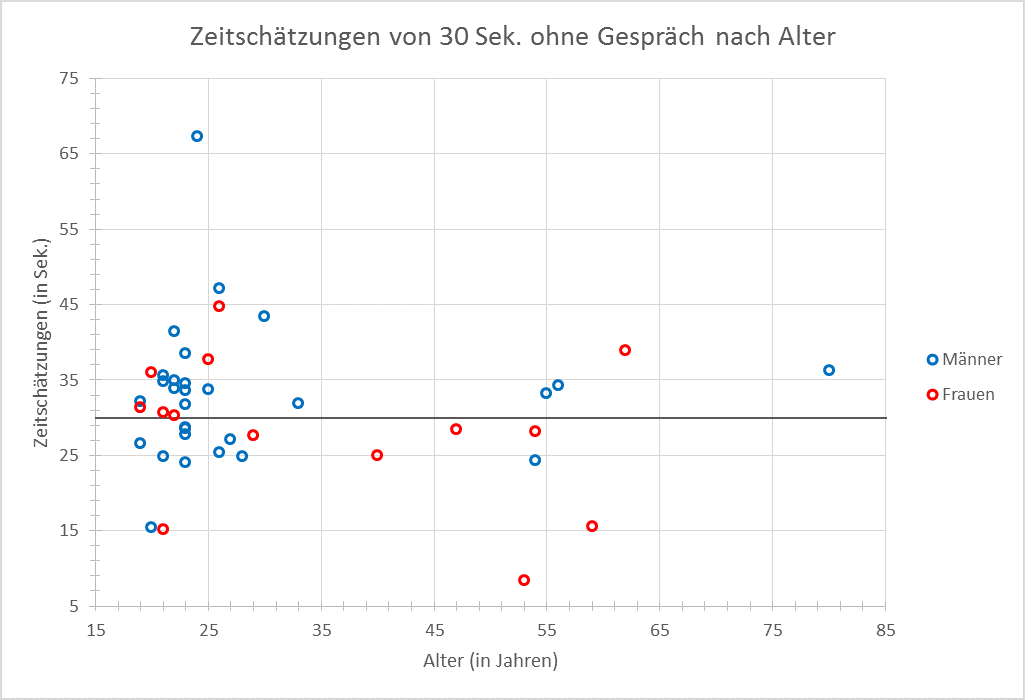
\includegraphics[scale=0.7]{../Diagramme/scatterPre/30ohne_alter.png}
	\caption{Zeiteinschätzungen von 30 Sek. ohne Gespräch nach Alter}
	\label{img:alter30ohne}
\end{figure}

\begin{figure}[H]
	\centering
	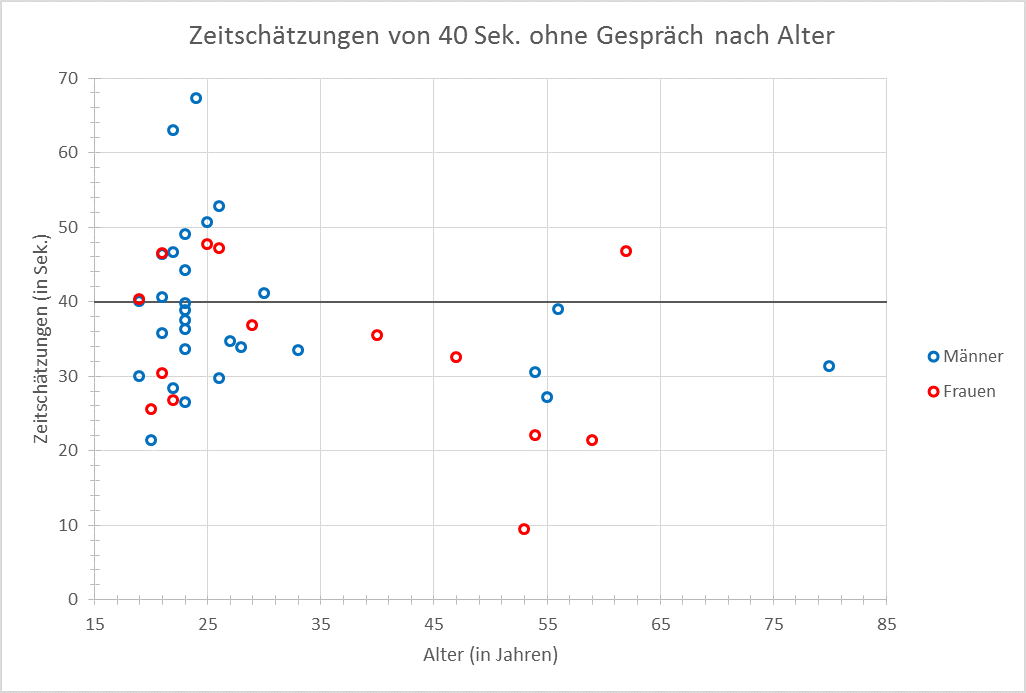
\includegraphics[scale=0.7]{../Diagramme/scatterPre/40ohne_alter.png}
	\caption{Zeiteinschätzungen von 40 Sek. ohne Gespräch nach Alter}
	\label{img:alter40ohne}
\end{figure}


Weder Abb. \ref{img:alter30ohne} noch Abb. \ref{img:alter40ohne} geben ein klares Bild zur Relation von Alter und Zeitempfinden, da die ermittelten Werte recht gleichmäßig verteilt sind. In beiden Einschätzungen gibt es Ausreißer in den Alterskategorien, in die viele Versuchspersonen fielen. Daher ist keine Abhängigkeit zwischen Zeiteinschätzung und der Variable ''Alter'' zu erkennen. %Es scheint hier ebenfalls keinen Unterschied zwischen Männern und Frauen zu geben. 


%%%%%%%%%%%%%%%%%%%%%%%%%%%%%%%%%%%%%%%%%%%%%%%%%%%%%%%% Intelligenz %%%%%%

\begin{figure}[H]
	\centering
	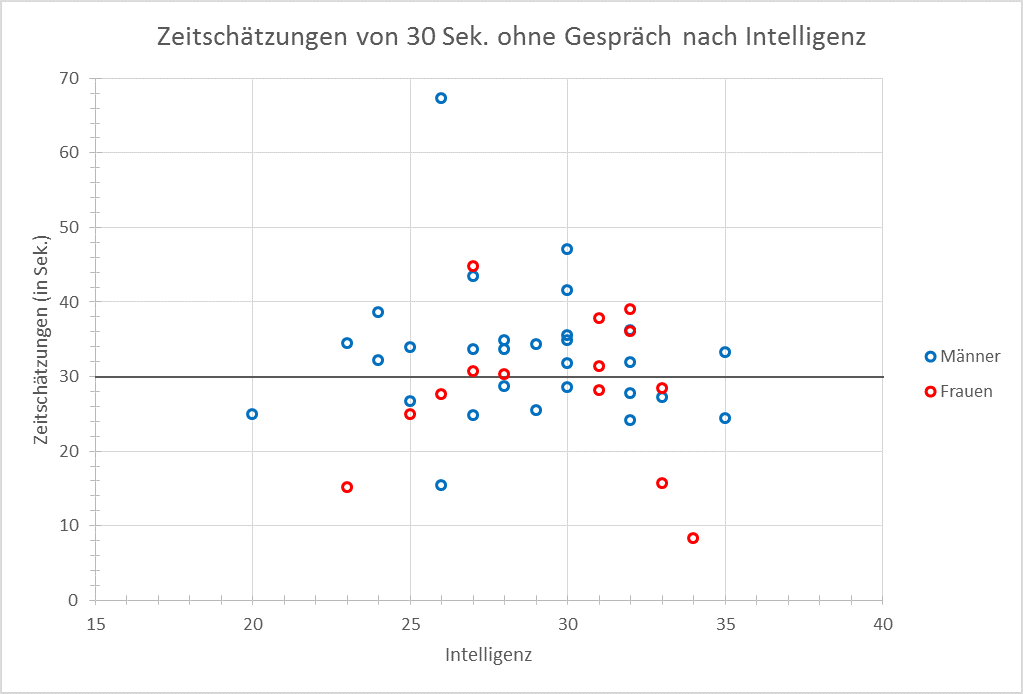
\includegraphics[scale=0.7]{../Diagramme/scatterPre/30ohne_intelligenz.png}
	\caption{Zeiteinschätzungen von 30 Sek. ohne Gespräch nach Intelligenz}
	\label{img:intell30ohne}
\end{figure}
\begin{figure}[H]
	\centering
	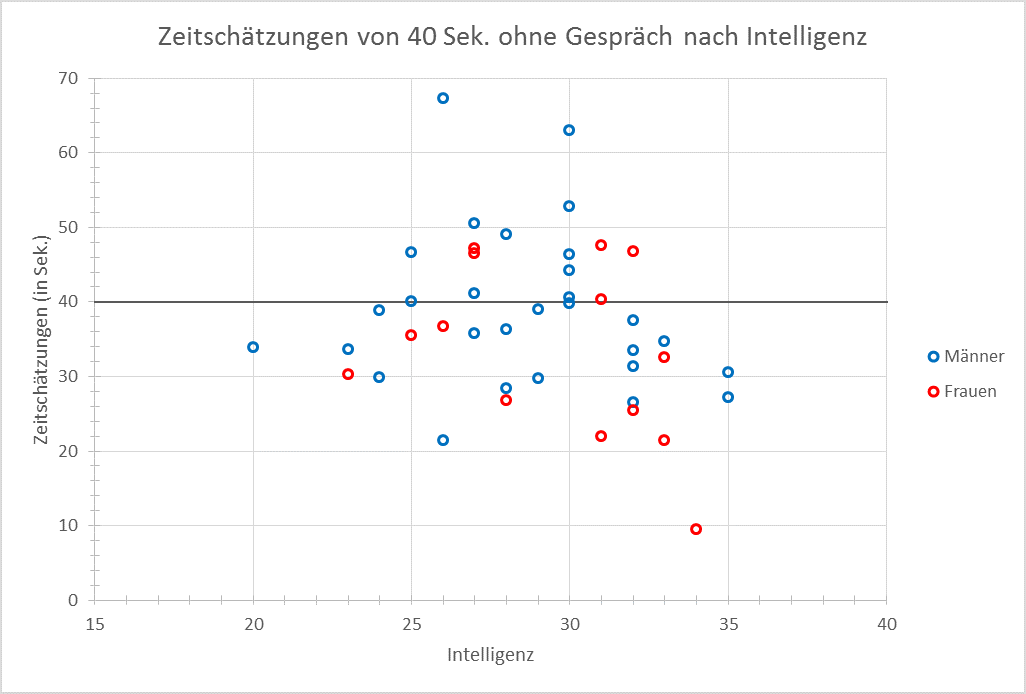
\includegraphics[scale=0.7]{../Diagramme/scatterPre/40ohne_intelligenz.png}
	\caption{Zeiteinschätzungen von 40 Sek. ohne Gespräch nach Intelligenz}
	\label{img:intell40ohne}
\end{figure}

Der verwendete Intelligenztest sieht folgende Verteilung vor: 0-5 Punkte (sehr niedrige Intelligenz), 6-20 Punkte (niedrige Intelligenz), 21-30 Punkte (durchschnittliche Intelligenz), 31-33 Punkte (hohe Intelligenz), 34-37 Punkte (sehr hohe Intelligenz). Die meisten Werte aus Abbildung \ref{img:intell30ohne} befinden sich  $+/-$10 Sekunden vom erwarteten Wert, allerdings sind auch die Ausreißer über alle Intelligenzklassen verteilt. Die erfassten Werte aus Abbildung \ref{img:intell40ohne} zeigen ebenfalls keine klare Tendenz und die Ausreißer sind auch hier gleichmäßig verteilt.  
Somit bleibt auch die Variable ,,Intelligenz'' ohne sichtbare Beziehung zu Zeitempfinden und die Vermutung, dass eine höhere Intelligenz auch mit einem besseren Zeiteinschätzungsvermögen verbunden ist, bleibt unbestätigt.



%%%%%%%%%%%%%% SCATTERPLOTS NACH TEMPERATUR



\begin{figure}[H]
	\centering
	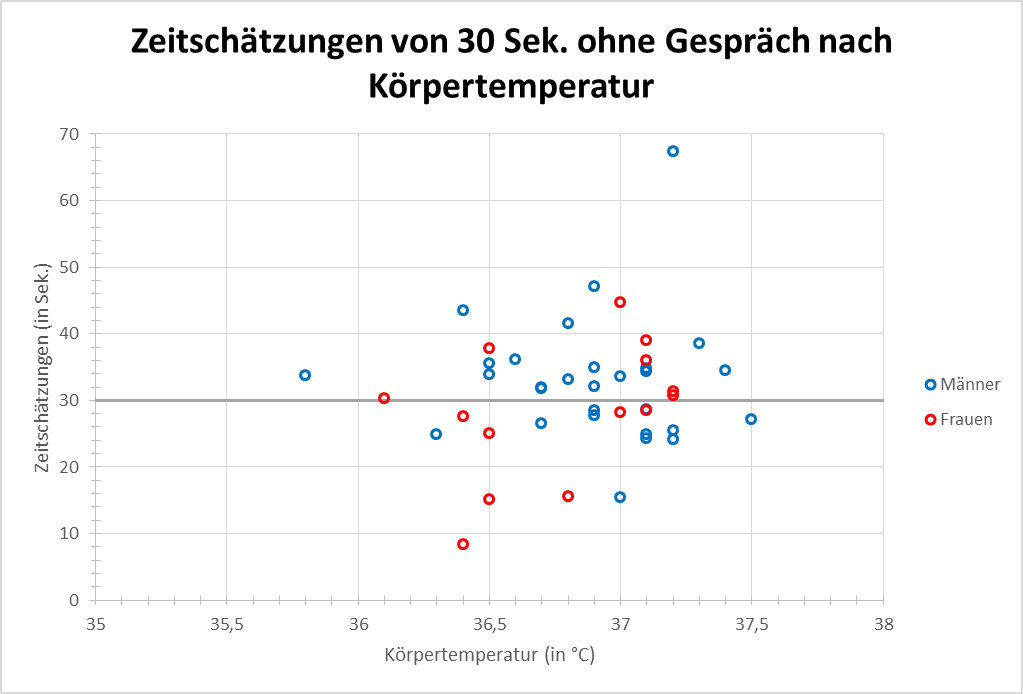
\includegraphics[scale=0.7]{../Diagramme/scatterPre/30ohne_koerpertemperatur.png}
	\caption{Zeiteinschätzungen von 30 Sek. ohne Gespräch nach Körpertemperatur}
	\label{img:temp30ohne}
\end{figure}
\begin{figure}[H]
	\centering
	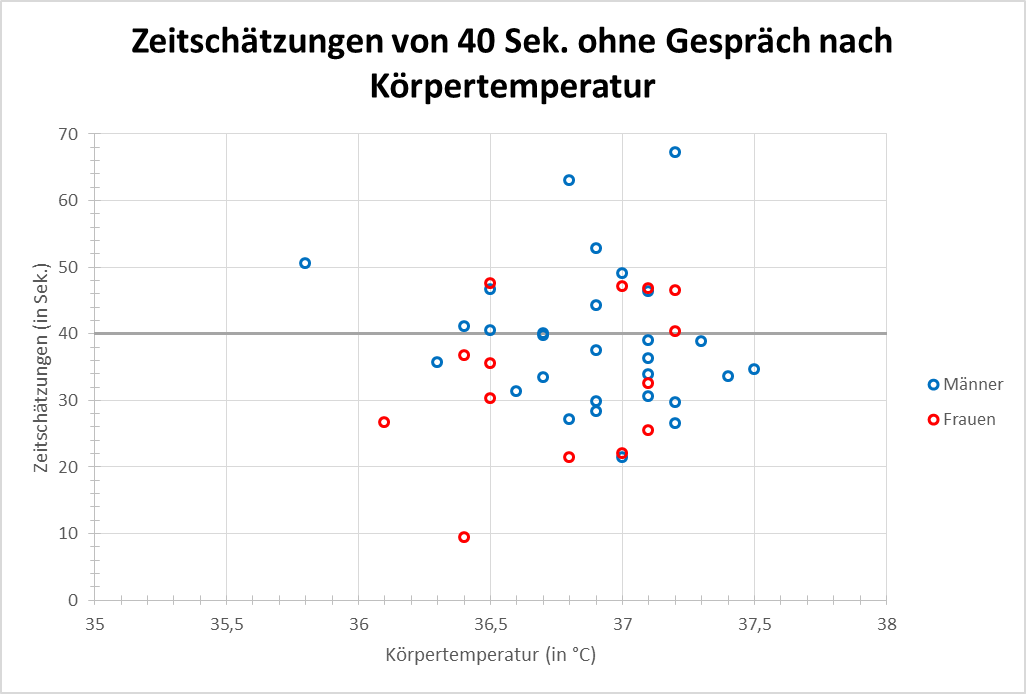
\includegraphics[scale=0.7]{../Diagramme/scatterPre/40ohne_koerpertemperatur.png}
	\caption{Zeiteinschätzungen von 40 Sek. ohne Gespräch nach Körpertemperatur}
	\label{img:temp40ohne}
\end{figure}


%%%%%%%%%%%%%%%%%%%%%%%%%%%%%%%%%%%%%%%%%%%%%%%%%%%%%%%% HISTO TEMP %%%%%%


 
Die stärksten Ausreißer aus Abb. \ref{img:temp30ohne} liegen sowohl knapp über als auch unter der Durchschnittstemperatur (36,83\textdegree C). Die Versuchspersonen, die weiter vom Durchschnitt entfernt liegen, scheinen die Zeit auch näher am Erwartungswert zu schätzen, allerdings muss auch hier beachtet werden, dass gerade hier die meisten Daten für Versuchspersonen zur Verfügung stehen. 
Gleichermaßen uneindeutig ist Abb. \ref{img:temp40ohne}, wobei hier noch mehr Einschätzungen vom Erwartungswert abweichen. 	
Dementsprechend kann man ebenfalls keinen Zusammenhang zwischen Körpertemperatur und Zeitempfinden feststellen. 


%%%%%%%%%%%%%%%%%%%%%%%%%%%%%%%%%%%%%%%%%%%%%%%%%%%%%%%% HISTO MÜDE %%%%%%
%%%%%%%%%%%%%%%%%%%
%%%%%%%%%%%%%%%%%%%%%%%%%%%%%%%%%%%%%%%%%%%%%%%%%%%%%%%%%%%%%%%%%%%%%%%%%%%%%%%%%%%%%%%%%

\begin{figure}[H]
	\centering
	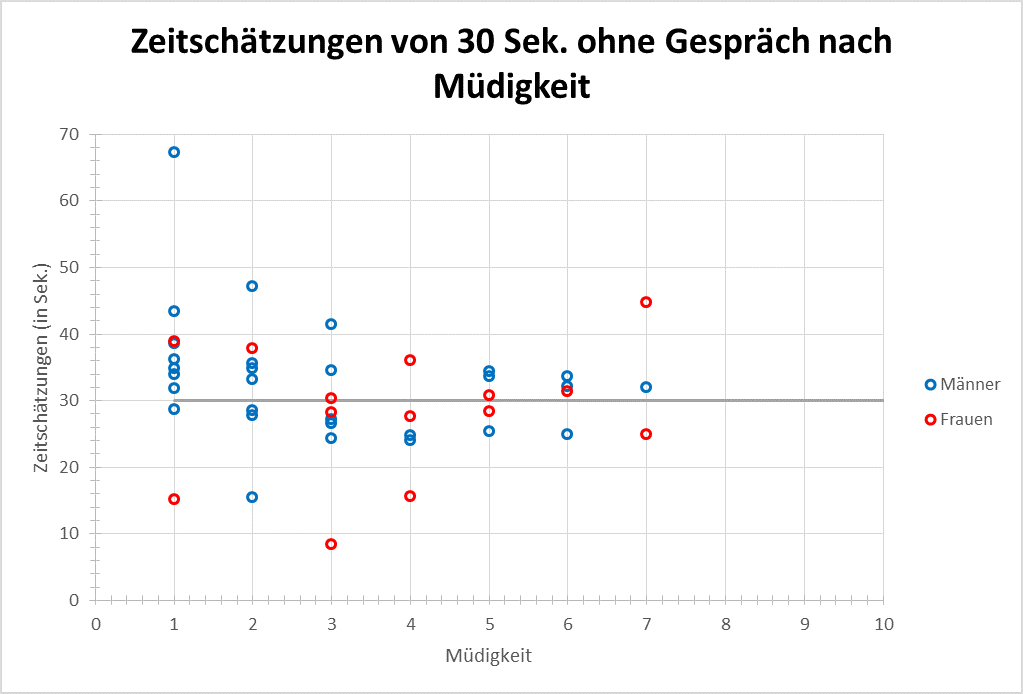
\includegraphics[scale=0.7]{../Diagramme/scatterPre/30ohne_muedigkeit.png}
	\caption{Zeiteinschätzungen von 30 Sek. ohne Gespräch nach Müdigkeit}
	\label{img:mued30ohne}
\end{figure}
\begin{figure}[H]
	\centering
	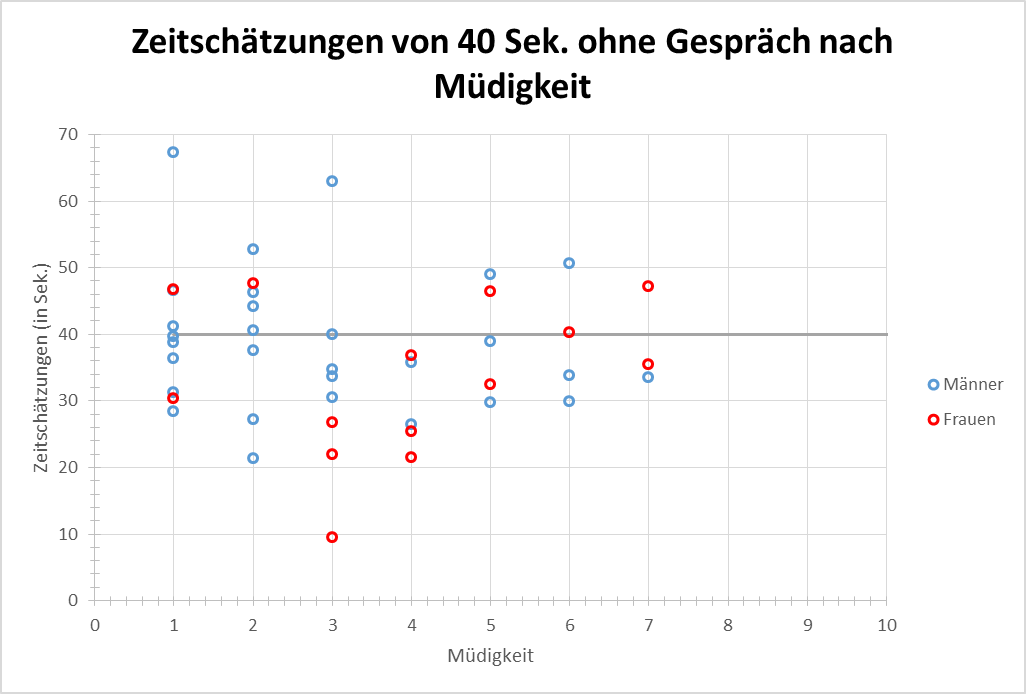
\includegraphics[scale=0.7]{../Diagramme/scatterPre/40ohne_muedigkeit.png}
	\caption{Zeiteinschätzungen von 40 Sek. ohne Gespräch nach Müdigkeit}
	\label{img:mued40ohne}
\end{figure}
Die Müdigkeitsskala erstreckt sich von 1 (nicht müde) bis 10 (sehr müde). Auffällig ist hier, dass ab einem mittleren Müdigkeitswert die Schätzungen aus Abb. \ref{img:temp30ohne}, bis auf eine Ausnahme, näher am Erwartungswert liegen. In Abb. \ref{img:mued40ohne} befinden sich die größten Ausreißer ebenfalls im Bereich 1 bis 4, allerdings stehen in diesem auch mehr  Daten zur Verfügung.\\

\subsubsection{Zeitschätzungen nach der VR}

\begin{figure}[H]
	\centering
	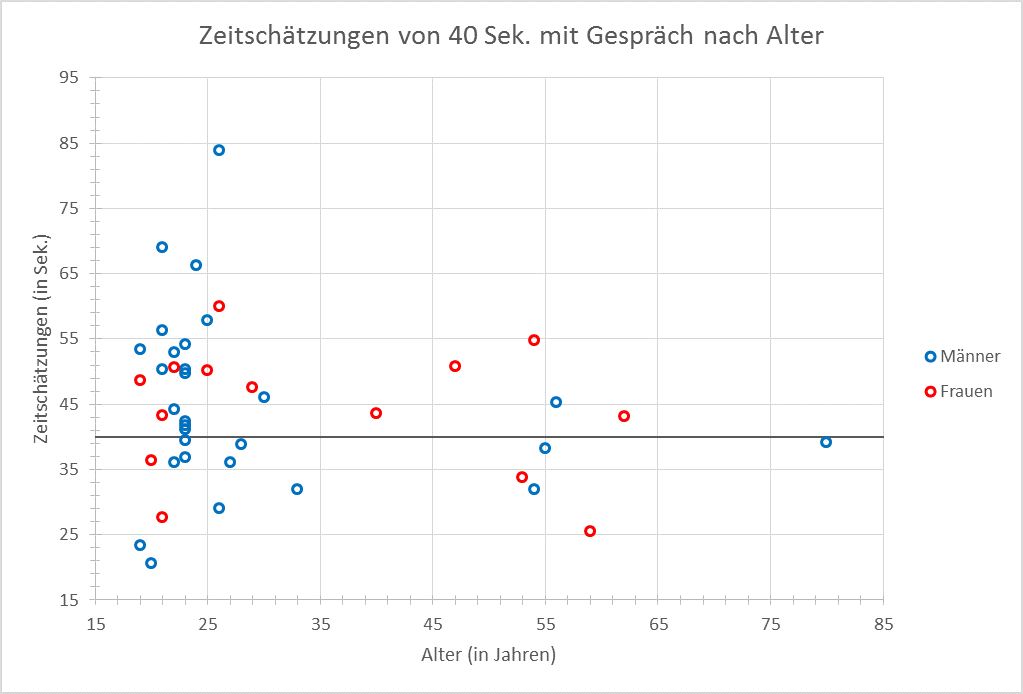
\includegraphics[scale=0.7]{../Diagramme/scatterPre/40mit_alter.png}
	\caption{Zeiteinschätzungen von 40 Sek. mit Gespräch nach Alter}
	\label{img:alter40mit}
\end{figure}

Die stärksten Abweichungen finden sich hier im Bereich der 20- bis 30-jährigen, allerdings stehen hier wieder die meisten Daten zur Verfügung. 


\begin{figure}[H]
	\centering
	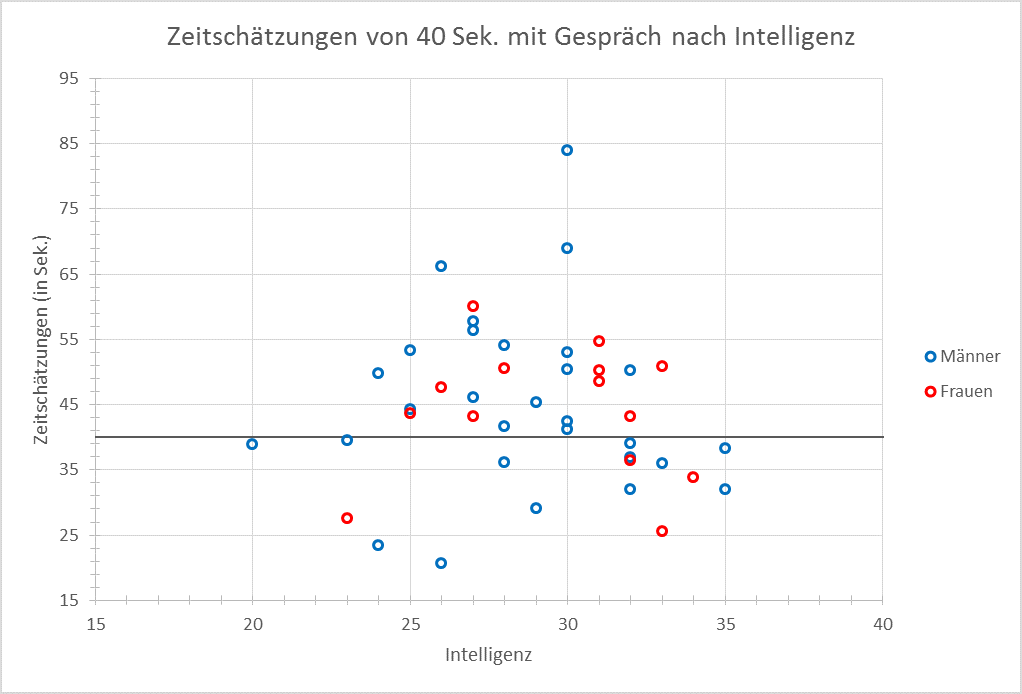
\includegraphics[scale=0.7]{../Diagramme/scatterPre/40mit_intelligenz.png}
	\caption{Zeiteinschätzungen von 40 Sek. mit Gespräch nach Intelligenz}
	\label{img:intell40mit}
\end{figure}

Viele der durchschnittlich intelligenten Versuchspersonen schätzen die tatsächlich verstrichene Zeit als kürzer ein, wohingegen jene mit niedrigerer und höherer Intelligenz näher am Erwartungswert liegen. Hierbei sei wieder angemerkt, dass hier die meisten Daten zur Verfügung stehen und nur eine Minderheit die Extreme auf beiden Seiten darstellt.

\begin{figure}[H]
	\centering
	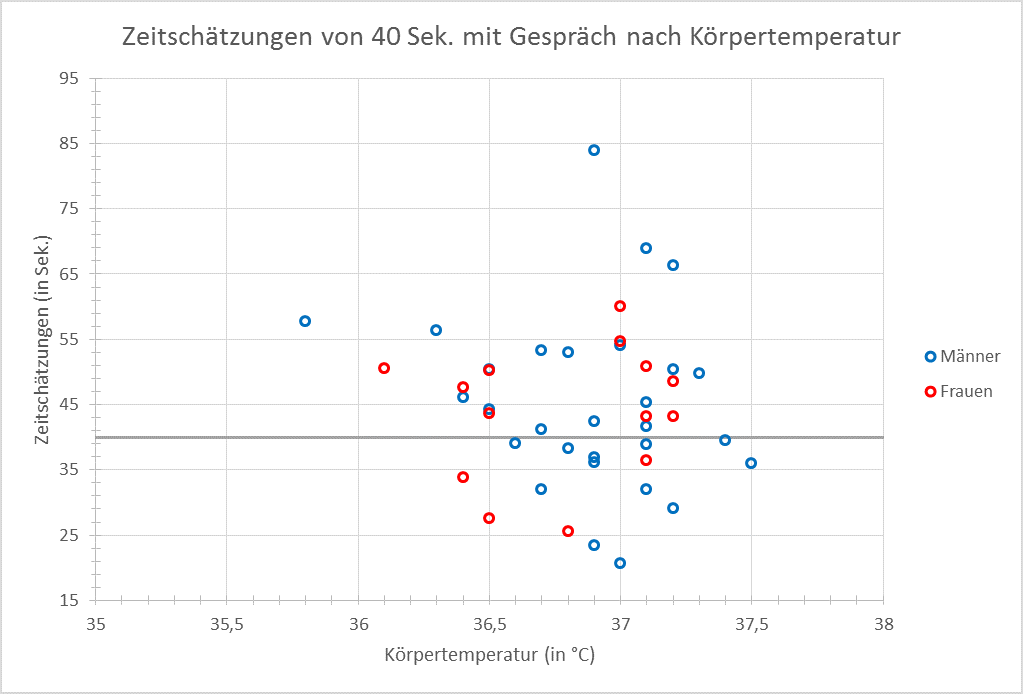
\includegraphics[scale=0.7]{../Diagramme/scatterPre/40mit_koerpertemperatur.png}
	\caption{Zeiteinschätzungen von 40 Sek. mit Gespräch nach Körpertemperatur}
	\label{img:temp40mit}
\end{figure}

%%%%%%%%%%%%%%%%%%%%%%%%%%%%%%%%%%%%%%%%%%%%%%%%%%%%%%%%%%%%%%%%%%%%%%%%%%%%%%%%%%%%%
Die stärksten Abweichungen finden sich hier in um die Durchschnittstemperatur (36,83\textdegree C).  Bei Versuchspersonen mit niedrigerer Temperatur gibt es ebenfalls, wenn auch nicht so starke, Abweichungen.



%%%%%%%%%%%%%%%%%%%%%%%%%%%%%%%%%%%%%%%%%%%%%%%%%%%%%%%%%%%%%%%%%%%%%%%%%%%%%%%%%%%%%


\begin{figure}[H]
	\centering
	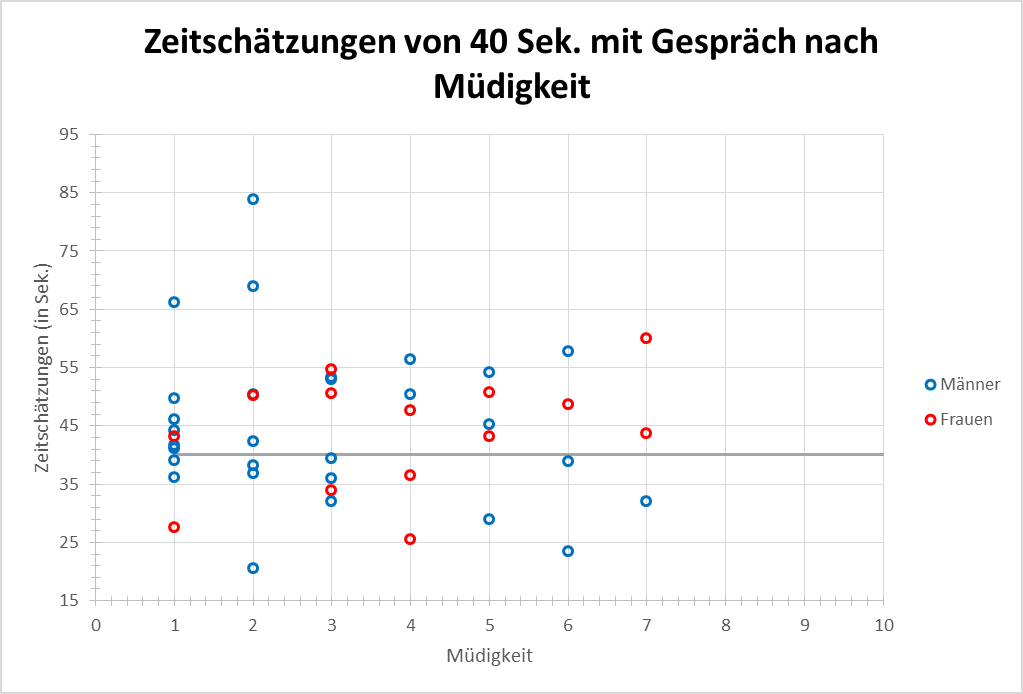
\includegraphics[scale=0.7]{../Diagramme/scatterPre/40mit_muedigkeit.png}
	\caption{Zeiteinschätzungen von 40 Sek. mit Gespräch nach Müdigkeit}
	\label{img:mued40mit}
\end{figure}

Ähnlich wie in den Einschätzungen ohne Gespräch liegen auch hier die stärksten Abweichungen im Bereich der Versuchspersonen, die weniger müde sind. Andererseits liegen die gemessenen Werte nicht näher am Erwartungswert, je müder die Versuchspersonen sind. Daher lässt sich auch hier kein Zusammenhang feststellen.\\
Im Allgemeinen kann man feststellen, dass keiner der berücksichtigten Einflussfaktoren in einem klaren Zusammenhang mit der Zeitwahrnehmung der Versuchspersonen steht.




\begin{figure}[H]
	\centering
	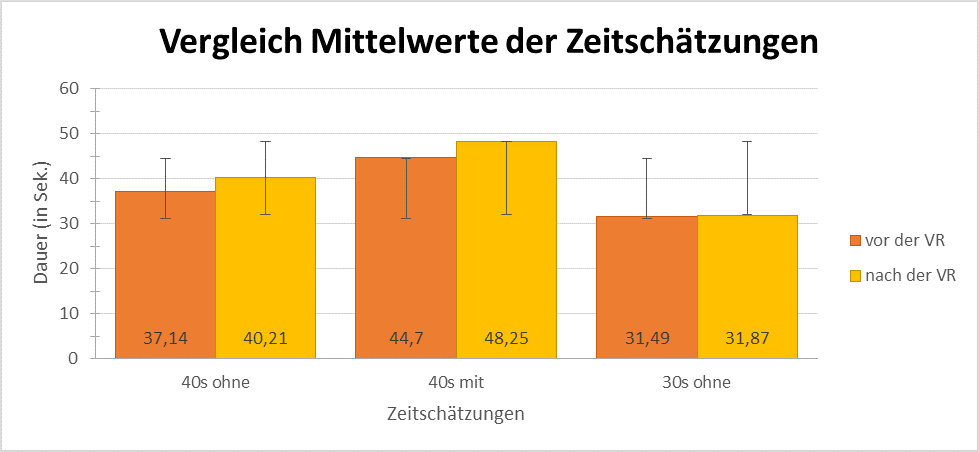
\includegraphics[scale=0.7]{../Diagramme/zeitschaetzungen/vergleich.png}
	\caption{Gesamtheit der Zeiteinschätzungen}
	\label{zeiteinschaetzungen}
\end{figure}


Es fällt auf, dass Versuchspersonen längere Zeitspannen (40 Sekunden) allgemein stärker überschätzten als kürzere (30 Sekunden). Diese längeren Zeitspannen wurden vor der VR um durchschnittlich 4,7 Sekunden und nach der VR sogar um 8,25 Sekunden überschätzt.
Im Bezug auf \textit{Hypothese 2} fällt auf, dass die längeren Zeitspannen nach der VR durchschnittlich stärker überschätzt wurden als vor der VR. Lediglich die 30 Sekunden wurden vor und nach der VR durchschnittlich annähernd gleich geschätzt. Entsprechend kann festgestellt werden, dass  eine leichte Verschlechterung im Abschätzen von 40 Sekunden (sowohl mit als auch ohne Gespräch) gemessen werden konnte, die VR keinen sehr eindeutigen Einfluss auf menschliches Zeitempfinden hat.
%%%%%%%%%%%%%%%%%%%%%%%%%%%%%%%%%%%%%%%%%%%%%%%%%%%%%

       



\section{Diskussion}

Ein Großteil unserer Untersuchungen hat zu keinem eindeutigen Ergebnis geführt. Lediglich die erste unserer drei Hypothesen ("`Visuelle und auditive Zeitgeber verändern das Zeitempfinden der Versuchsperson in der virtuellen Welt'') hat sich zum Teil bestätigt -- insbesondere die auditiven Zeitgeber haben eine Beeinflussung gezeigt. Das Zeitempfinden der Versuchspersonen hat sich nach dem VR-Aufenthalt nur sehr geringfügig verändert und es war keine Beziehung zwischen Spaß- und Zeitempfinden zu erkennen.
 
Ein Grund für die wenigen positiven Ergebnisse kann sein, dass eine größere Anzahl von Versuchspersonen oder zumindest eine gleichmäßigere Verteilung (z.B.\ zwischen dem Männer- und Frauenanteil oder den Altersstufen) notwendig gewesen wäre.

Als Intelligenztest wurde lediglich eine Kurzform verwendet, der zudem stark mit den sprachlichen Fähigkeiten der jeweiligen Versuchsperson zusammenhing (vor allem für Nicht-Muttersprachler eine Schwierigkeit). Es wäre möglich, die Intelligenz vor dem Experiment noch exakter zu überprüfen, auch wenn dies die Gesamtdauer des Experiments erheblich verlängern würde.

Die Einteilung der Müdigkeitsstufen erfolgte nach Selbsteinschätzung, die keine vollkommene Zuverlässigkeit erreichen kann. Hier könnte auf Methoden wie z.B.\ das Zählen von Wimpernschlägen zurückgegriffen werden, um an exaktere Werte zu gelangen.

Auch ungenaue Messungen/Messfehler (z.B.\ bei der Körpertemperatur) können in Einzelfällen nicht ausgeschlossen werden und einen Einfluss auf unser Ergebnis genommen haben.

Eine weiterer Grund für die nicht bestätigten Hypothesen ist, dass die Zeitintervalle der einzelnen Szenarien nicht direkt, während sich die Versuchsperson in der VR-Welt befunden hatte, sondern erst im Nachhinein eingeschätzt werden mussten.
Somit wurde nicht nur die Fähigkeit, Zeit richtig einschätzen zu können, sondern
ebenfalls das Erinnerungsvermögen gefordert, was nicht Ziel unserer Untersuchung sein sollte. Dies sollte bei einer weiteren Durchführung des Experiment unbedingt verändert werden (d.h.\ es sollten unmittelbare Zeiteinschätzungen während des VR-Aufenthalt erfolgen).

Definitiv verändert werden müssen bei einer weiteren Durchführung zudem die gewählten Zeitspannen für Schätzung der Gesamtdauer des VR-Aufenthalts. Eine Versuchsperson hielt sich durchschnittlich 238 Sekunden in der VR-Welt auf -- die erste auswählbare Zeitspanne von 0-7 Minuten war bereits viel zu groß definiert. Dadurch sind die erlangten Ergebnisse nicht aussagekräftig.


\newpage

\printbibliography

\begin{appendix}
\section{Anhang}

\subsection{3D-Objekte}

\subsubsection{American Store}

\textbf{used textures (all licences acquired):}
(last viewed: yyyy-mm-dd)

air\_conditioning:
https://www.textures.com/download/aircos0097/63182?q=air+con
(last viewed: 2017-07-14)

asphalt\_damaged:
https://www.textures.com/download/asphaltdamaged0059/46538?q=asphalt+damaged
(last viewed: 2017-07-14)

back\_door:
https://www.textures.com/download/doorswood0128/64000?q=DoorsWood0128
(last viewed: 2017-07-14)

brown\_concrete:
https://www.textures.com/download/substance0066/128441?q=concrete+brown
(last viewed: 2017-07-14)

concrete\_bare2:
https://www.textures.com/download/concretebare0280/35243?q=ConcreteBare0280
(last viewed: 2017-07-14)

front\_door:
https://www.textures.com/download/doorswood0125/50420?q=door
(last viewed: 2017-07-14)

glas:
https://www.textures.com/download/windowsother0014/44984?q=WindowsOther0014
(last viewed: 2017-07-14)

metal\_plates:
https://www.textures.com/download/metalplatesbare0154/123165?q=MetalPlatesBare0154
(last viewed: 2017-07-14)

plywood\_painted-green:
https://www.textures.com/download/plywoodpainted0024/5719?q=plywood+painted
(last viewed: 2017-07-14)

plywood\_painted-white:
https://www.textures.com/download/plywoodpainted0057/59134?q=plywood+painted+white
(last viewed: 2017-07-14)

rough\_bricks:
https://www.textures.com/download/3dscans0037/126993?q=rough+bricks
(last viewed: 2017-07-14)

rubber:
https://www.textures.com/download/rubber0044/58887?q=Rubber0044
(last viewed: 2017-07-14)

shutter:
https://www.textures.com/download/windowsshutters0096/31421?q=WindowsShutters0096
(last view: 2017-07-14)

soilsand:
https://www.textures.com/download/soilsand0210/61549?q=soilsand0210
(last viewed: 2017-07-14)
---
\textbf{used normalmap:}

all normalmaps were created out of the respective textures using 'http://cpetry.github.io/NormalMap-Online/'
(last viewed: 2017-07-14)

\subsubsection{Straßenverkehr}

strassenoberfläche:
http://www.bildburg.de/texturen/boden/strassen/
(last viewed: 2017-07-20)


%%%%%%%%%%%%%%%%% Alinas Texturen %%%%%%%%%%%%%%%%%%%%%%%%%%%%%%%%% 
https://pixabay.com/de/textur-stamm-holz-nahaufnahme-1411201/



https://pixabay.com/de/textur-baum-rinde-hintergrund-2119288/



https://pixabay.com/de/mauer-steine-wand-hauswand-450106/



https://pixabay.com/de/wand-putz-hintergrund-fassade-2146911/



https://pixabay.com/de/t\%C3\%BCr-alt-eingang-die-alte-t\%C3\%BCr-2166761/



https://pixabay.com/de/die-t\%C3\%BCr-holz-burg-blumen-t\%C3\%BCrgriff-1908710/



https://pixabay.com/de/die-t\%C3\%BCr-holz-burg-blumen-t\%C3\%BCrgriff-1909077/



https://pixabay.com/de/dach-ziegel-bunt-rot-dachplatten-1197886/



https://pixabay.com/de/dachziegel-dachpfannen-dach-707888/



https://pixabay.com/de/dachziegel-dachpfannen-dach-1301459/



https://pixabay.com/de/dach-bretter-holzwand-holz-2071600/



https://pixabay.com/de/hauswand-ziegelsteine-backsteine-298039/



https://pixabay.com/de/steinwand-stein-mauer-wand-2370933/



https://pixabay.com/de/blatt-gr\%C3\%BCn-gr\%C3\%BCnes-blatt-910532/



https://pixabay.com/de/herbst-herbstbl\%C3\%A4tter-laub-1655915/



https://pixabay.com/de/erdbeeren-erdbeere-lecker-obst-1326148/



https://pixabay.com/de/gem\%C3\%BCse-gurke-tomaten-kirschtomate-1940461/

\end{appendix}

\vfill %Zum Seitenende Verschieben


\end{document}
